\documentclass[11pt,a4paper]{article}
\usepackage[T1]{fontenc}
\usepackage[utf8]{inputenc}
\usepackage{charter}
\usepackage[scaled=0.92]{sourcesanspro}
\usepackage[charter]{mathdesign}
\usepackage{microtype}
\usepackage[margin=2.3cm,headheight=14pt]{geometry}
\usepackage{xcolor}
\usepackage{graphicx}
\usepackage{booktabs,tabularx,array}
\usepackage{enumitem}
\usepackage{multicol}
\usepackage{amsmath}
\usepackage{titlesec}
\usepackage{fancyhdr}
\usepackage[most]{tcolorbox}
\usepackage{tikz}
\usetikzlibrary{arrows.meta,positioning,calc,shapes.geometric,decorations.pathmorphing,patterns,backgrounds,fit}
\usepackage{pgfplots}
\pgfplotsset{compat=1.18}
\usepgfplotslibrary{groupplots}
\usepackage[hidelinks]{hyperref}

% ------------------------------------------------------------------ colours
\definecolor{ink}{HTML}{1F2A37}
\definecolor{navy}{HTML}{1F4E79}
\definecolor{teal}{HTML}{1B7F79}
\definecolor{amber}{HTML}{C17C00}
\definecolor{brick}{HTML}{A23B2A}
\definecolor{slate}{HTML}{5B6573}
\definecolor{mist}{HTML}{EEF3F8}
\definecolor{sand}{HTML}{FBF5E9}
\definecolor{cP1}{HTML}{1F4E79}
\definecolor{cP2}{HTML}{8DA9C4}
\definecolor{cP3}{HTML}{1B7F79}
\definecolor{cP4}{HTML}{C17C00}
\color{ink}

% ------------------------------------------------------------------ headings
\titleformat{\section}{\sffamily\Large\bfseries\color{navy}}{\thesection}{0.8em}{}[\vspace{-0.4em}{\color{navy!25}\rule{\linewidth}{0.6pt}}]
\titleformat{\subsection}{\sffamily\large\bfseries\color{navy}}{\thesubsection}{0.7em}{}
\titlespacing*{\section}{0pt}{1.6em}{0.9em}
\titlespacing*{\subsection}{0pt}{1.2em}{0.5em}
\pagestyle{fancy}\fancyhf{}
\fancyhead[L]{\sffamily\footnotesize\color{slate}Clinical Resilience over UAV-Assisted LEO Backhaul: A Beginner's Tutorial}
\fancyhead[R]{\sffamily\footnotesize\color{slate}\thepage}
\renewcommand{\headrulewidth}{0.3pt}
\setlength{\parindent}{0pt}\setlength{\parskip}{0.55em}
\setlist{itemsep=0.2em,topsep=0.3em}

% ------------------------------------------------------------------ boxes
\newtcolorbox{term}[1]{enhanced,breakable,colback=mist,colframe=navy,boxrule=0pt,leftrule=2.5pt,arc=0pt,
  left=8pt,right=8pt,top=5pt,bottom=5pt,fonttitle=\sffamily\bfseries\small,coltitle=navy,
  title={Key terms: #1},attach title to upper={\par\smallskip},before skip=0.8em,after skip=0.8em}
\newtcolorbox{idea}{enhanced,breakable,colback=sand,colframe=amber,boxrule=0pt,leftrule=2.5pt,arc=0pt,
  left=8pt,right=8pt,top=5pt,bottom=5pt,fontupper=\small,before skip=0.8em,after skip=0.8em}
\newtcolorbox{example}[1][Worked example]{enhanced,breakable,colback=white,colframe=teal,boxrule=0.6pt,arc=2pt,
  left=8pt,right=8pt,top=5pt,bottom=5pt,fonttitle=\sffamily\bfseries\small,colbacktitle=teal!12,coltitle=teal!70!black,
  title={#1},before skip=0.8em,after skip=0.8em}
\newcommand{\kt}[1]{\textbf{\color{navy}#1}}
\newcommand{\insight}[1]{\begin{idea}\textsf{\textbf{\color{amber!80!black}Take-away.}} #1\end{idea}}

\begin{document}

% ================================================================== title
\begin{tikzpicture}[remember picture,overlay]
\fill[navy] (current page.north west) rectangle ([yshift=-5.2cm]current page.north east);
\node[anchor=north west,text width=15.5cm,align=left,text=white] at ([xshift=2.3cm,yshift=-1.3cm]current page.north west)
{\sffamily\small TUTORIAL FOR STUDENTS\\[4pt]
 \sffamily\bfseries\LARGE Can a Drone and a Satellite Keep a Patient Safe?\\[6pt]
 \sffamily\large Remote patient monitoring over a UAV-assisted LEO satellite link,\\ explained step by step};
\end{tikzpicture}
\vspace*{4.4cm}

{\sffamily\small\color{slate}
Based on: M.\,I.\ Younas, M.\,J.\ Iqbal, A.\,H.\ Sodhro, M.\ Iqbal and J.-Y.\ Pan, ``Toward Clinical Resilience of Remote Patient Monitoring over UAV-Assisted LEO Backhaul under Coverage Gaps, Jamming and Denial of Service,'' \emph{SUNRISE 2026}, Springer CCIS (in press).\\[2pt]
Prepared by Engr.\ Muhammad Irfan Younas, Department of Computer Systems Engineering, Sukkur IBA University.\par}

\begin{idea}
\textsf{\textbf{How to read this tutorial.}} No background in satellites or 5G is assumed. Every technical word is explained the first time it appears, in a blue \emph{Key terms} box. Yellow boxes give the main take-away of each section, and green boxes walk through small calculations. A full glossary (Section~\ref{sec:glossary}) and some self-test questions (Section~\ref{sec:quiz}) are at the end.
\end{idea}

\tableofcontents

% ================================================================== 1
\section{The Story Behind the Paper}

Imagine a small health centre in a village of the Tharparkar desert in Sindh. Ten heart patients wear small sensors. The nearest cardiologist works in a hospital in Karachi, more than 300\,km away, and there is no mobile-phone tower nearby. How can the doctor see the patients' heart signals in real time, and, more importantly, how can the doctor be warned \emph{immediately} if a patient's heart goes into a dangerous rhythm?

The paper studies one possible answer: a \kt{drone} hovers above the village, picks up the patients' data, and sends it up to a \kt{satellite}, which sends it down to a ground station near Karachi, from where it travels to the hospital over an ordinary cable network. The question the paper asks is simple to state:

\begin{center}
\begin{tcolorbox}[colback=white,colframe=navy,width=0.86\linewidth,arc=2pt,boxrule=0.8pt,halign=center]
\sffamily When things go wrong (the satellite disappears for a while, someone jams the radio, or a hacker floods the network), do the patients' alarms and heart signals still reach the doctor \emph{in time}?
\end{tcolorbox}
\end{center}

The answer, as we will see, is ``it depends'': the paper finds out \emph{what} it depends on, and by how much.

\begin{term}{the setting}
\kt{Remote patient monitoring (RPM)}: watching a patient's health (heart rate, ECG, oxygen, etc.) from a distance, while the patient stays at home or in a local clinic.\par
\kt{IoMT (Internet of Medical Things)}: medical devices (wearable sensors, monitors) that are connected to a network and send data automatically.\par
\kt{ECG (electrocardiogram)}: the electrical signal of the heart, the familiar wavy line on a heart monitor.\par
\kt{Hub (gateway)}: a small box in the clinic that collects data from all the patients' sensors and sends it onward. In the paper it acts like a mobile phone.\par
\kt{UAV (unmanned aerial vehicle)}: a drone. Here it acts like a flying mobile-phone tower and relay.\par
\kt{Backhaul}: the long-distance connection that carries data from a local network to the wider internet or, here, to the hospital.
\end{term}

% ================================================================== 2
\section{The Delivery Path, One Hop at a Time}

Figure~\ref{fig:path} shows the full chain. Each arrow is called a \kt{hop}, because data ``hops'' from one device to the next.

\begin{figure}[h]
\centering
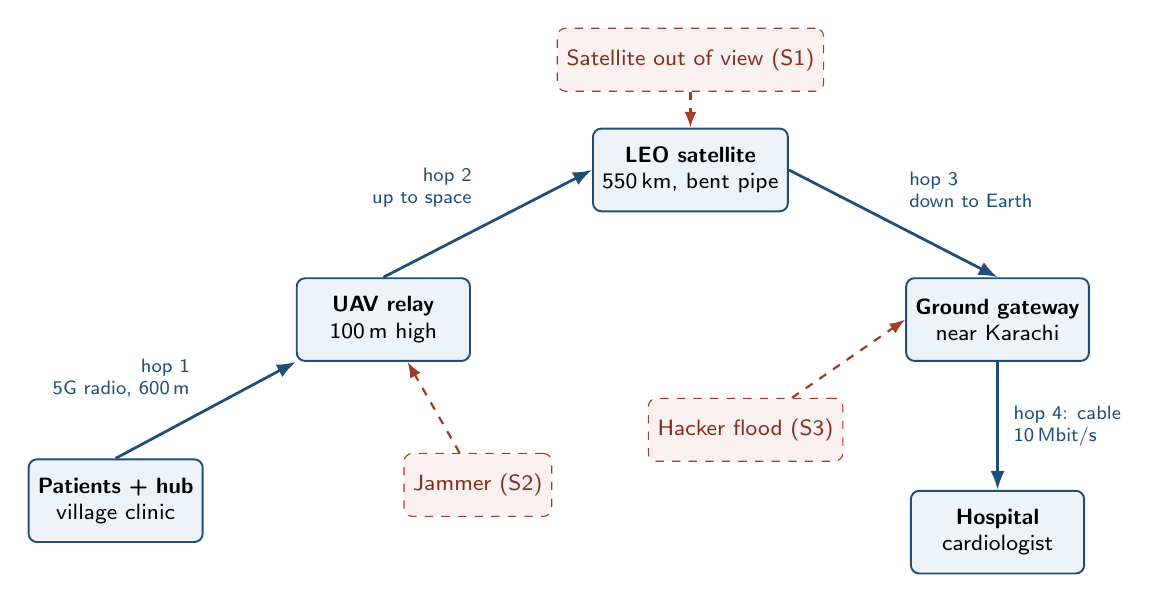
\begin{tikzpicture}[font=\sffamily\footnotesize,
  dev/.style={draw=navy,fill=mist,rounded corners=3pt,minimum width=2.2cm,minimum height=1.05cm,align=center,line width=0.7pt},
  bad/.style={draw=brick,fill=brick!7,dashed,rounded corners=3pt,minimum height=0.8cm,align=center,text=brick!80!black},
  hop/.style={-{Latex[length=2.4mm]},line width=1pt,navy},
  atk/.style={-{Latex[length=2mm]},dashed,brick,line width=0.8pt}]
\node[dev] (hub) at (0,0) {\textbf{Patients + hub}\\village clinic};
\node[dev] (uav) at (3.4,2.3) {\textbf{UAV relay}\\100\,m high};
\node[dev] (sat) at (7.3,4.2) {\textbf{LEO satellite}\\550\,km, bent pipe};
\node[dev] (gw)  at (11.2,2.3) {\textbf{Ground gateway}\\near Karachi};
\node[dev] (hos) at (11.2,-0.4) {\textbf{Hospital}\\cardiologist};
\draw[hop] (hub.north) -- node[above left=1pt and 2pt,pos=0.5,align=right,font=\sffamily\scriptsize,text=navy]{hop 1\\5G radio, 600\,m} (uav.south west);
\draw[hop] (uav.north) -- node[above left=2pt and 2pt,pos=0.5,align=right,font=\sffamily\scriptsize,text=navy]{hop 2\\up to space} (sat.west);
\draw[hop] (sat.east) -- node[above right=2pt and 2pt,pos=0.5,align=left,font=\sffamily\scriptsize,text=navy]{hop 3\\down to Earth} (gw.north);
\draw[hop] (gw) -- node[right=2pt,align=left,font=\sffamily\scriptsize,text=navy]{hop 4: cable\\10\,Mbit/s} (hos);
\node[bad] (jam) at (4.6,0.2) {Jammer (S2)};
\node[bad] (dos) at (8.0,0.9) {Hacker flood (S3)};
\node[bad] (gap) at (7.3,5.6) {Satellite out of view (S1)};
\draw[atk] (jam) -- (uav);
\draw[atk] (dos) -- (gw.west);
\draw[atk] (gap) -- (sat);
\end{tikzpicture}
\caption{The delivery path studied in the paper. Solid arrows carry patient data; dashed red boxes are the three kinds of trouble that are tested.}\label{fig:path}
\end{figure}

\begin{enumerate}
\item \textbf{Hub to UAV (hop 1).} The hub sends data by 5G radio to a drone hovering 100\,m up and 600\,m away. This is a short link, so the hub can use little power.
\item \textbf{UAV to satellite (hop 2).} The drone carries a satellite antenna and passes the data up to a \kt{LEO} satellite.
\item \textbf{Satellite to ground gateway (hop 3).} The satellite does not process the data; it simply amplifies it and sends it back down. This is called a \kt{bent pipe}.
\item \textbf{Gateway to hospital (hop 4).} A normal wired internet link of 10\,Mbit/s.
\end{enumerate}

\begin{term}{satellites and networks}
\kt{LEO (low Earth orbit)}: satellites flying only a few hundred kilometres up (here 550\,km). They are close, so delay is small, but they move fast and each one is overhead for only a few minutes.\par
\kt{Constellation} or \kt{shell}: a group of identical satellites at the same height, arranged so that together they cover the Earth. More satellites give better coverage.\par
\kt{Walker-delta constellation}: a standard, evenly spaced arrangement. ``53$^\circ$:528/24/1'' means: orbits tilted 53$^\circ$ to the equator, 528 satellites in 24 orbital planes (22 per plane), and phasing factor 1 (how neighbouring planes are offset).\par
\kt{Bent pipe (transparent satellite)}: the satellite works like a mirror in the sky; it does not decode the data.\par
\kt{Ground gateway}: the satellite dish on the ground that receives the data back from space. In a bent pipe, the UAV \emph{and} the gateway must see the \emph{same} satellite at the same time.\par
\kt{SAGIN (space-air-ground integrated network)}: a network that combines satellites (space), drones or planes (air) and normal towers or cables (ground), exactly like Figure~\ref{fig:path}.\par
\kt{5G NR (New Radio)}: the radio technology of 5G mobile networks.\par
\kt{NTN (non-terrestrial network)}: 5G delivered through satellites or high-flying platforms instead of towers.\par
\kt{3GPP}: the international body that writes the mobile-network standards (4G, 5G). Its technical reports are called \kt{TR} (e.g., TR~22.826) and its specifications \kt{TS}.
\end{term}

% ================================================================== 3
\section{What Data Is Sent, and What Counts as ``On Time''}

Not all medical data is equally urgent. The paper divides it into three \kt{traffic classes}:

\begin{center}
\small
\begin{tabularx}{0.96\linewidth}{@{}>{\bfseries}l X X@{}}
\toprule
Class & What it is & How fast it must arrive \\
\midrule
C1 Alarm & A short warning (100 bytes) when a sensor detects danger, e.g.\ an abnormal heart rhythm. About one per patient every 5 minutes, at random times. & Within \textbf{100\,ms} (one tenth of a second). \\
C2 ECG & A continuous heart signal: a 150-byte message every half second from each patient. & Each message within \textbf{100\,ms}; the stream must never stop for more than about \textbf{1\,s}. \\
C3 Record & A 1\,MB file (e.g., a full recording or report) every 10 minutes, cut into 1\,kB pieces. & Before the next file is due, i.e.\ within \textbf{600\,s}. \\
\bottomrule
\end{tabularx}
\end{center}

The 100\,ms and 1\,s numbers are not invented by the authors. They come from 3GPP TR~22.826, a 3GPP report that lists what communication networks must deliver for medical applications, in this case heart monitoring outside the hospital.

\begin{term}{time and reliability}
\kt{Latency (delay)}: the time from when a message is created until it arrives. 1\,ms = one thousandth of a second.\par
\kt{Deadline}: the latest acceptable arrival time. A message that arrives after it is counted as a \kt{deadline miss}, even if it arrives eventually.\par
\kt{Survival time}: how long the application can cope without receiving the next expected message before it is treated as a failure (here 1\,s).\par
\kt{Availability}: the share of time the service works. ``99.9999\,\%'' (``six nines'') allows only about 32 seconds of failure per year. Following TR~22.826, the ECG stream is counted as unavailable whenever an expected message has not arrived within 100\,ms + 1\,s = \textbf{1.1\,s}.\par
\kt{Poisson process}: the standard model of events that happen ``randomly and independently'', like phone calls arriving at a call centre. Alarms are modelled this way.\par
\kt{Bytes and bit rate}: 1 byte = 8 bits. A link of 10\,Mbit/s carries 10 million bits per second.
\end{term}

\insight{The paper does not ask ``how fast is the link on average?'' It asks ``does \emph{each} alarm and \emph{each} ECG message arrive within its medical deadline?'' Averages can look fine while individual alarms are dangerously late.}

% ================================================================== 4
\section{Three Things That Can Go Wrong}

The paper tests the path in four situations, called \kt{scenarios}. S0 is the normal case, and S1--S3 are the three problems.

\subsection{S1: The satellite goes out of view (coverage gaps)}

A LEO satellite crosses the sky in a few minutes. The UAV can only use a satellite that is high enough above the horizon; the paper uses 25$^\circ$. If there are few satellites in the constellation, there will be moments when \emph{no} satellite is high enough over both the UAV and the gateway. That period is a \kt{coverage gap}, and during it nothing can be sent.

\begin{figure}[h]
\centering
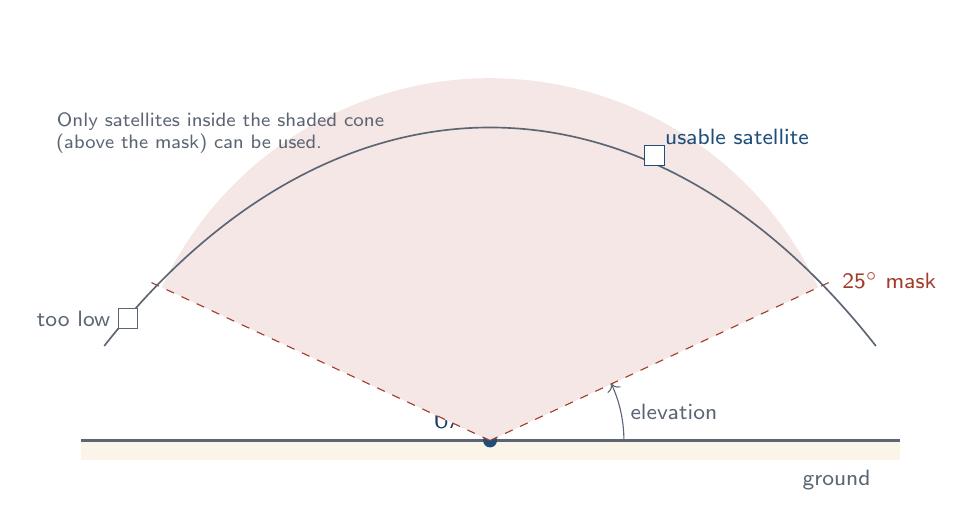
\begin{tikzpicture}[font=\sffamily\footnotesize]
\fill[sand] (-5.2,0) rectangle (5.2,-0.25);
\draw[line width=1pt,slate] (-5.2,0) -- (5.2,0);
\node[below,slate] at (4.4,-0.25) {ground};
\fill[navy] (0,0) circle (2.5pt) node[above left=1pt,navy!80!black]{UAV};
\fill[brick!12] (0,0) -- (25:4.6) arc (25:155:4.6) -- cycle;
\draw[dashed,brick] (0,0) -- (25:4.8) node[right,brick]{25$^\circ$ mask};
\draw[dashed,brick] (0,0) -- (155:4.8);
\draw[->,slate] (1.7,0) arc (0:25:1.7) node[midway,right,slate]{elevation};
\draw[slate,line width=0.6pt] (-4.9,1.2) .. controls (-2,4.9) and (2,4.9) .. (4.9,1.2);
\node[draw=navy,fill=white,minimum size=7pt,inner sep=0] at (60:4.18) {};
\node[navy,above right] at (60:4.2) {usable satellite};
\node[draw=slate,fill=white,minimum size=7pt,inner sep=0] at (-4.6,1.55) {};
\node[slate,left] at (-4.7,1.55) {too low};
\node[text width=4.6cm,align=left,font=\sffamily\scriptsize,slate] at (-3.2,3.9) {Only satellites inside the shaded cone (above the mask) can be used.};
\end{tikzpicture}
\caption{Elevation angle and elevation mask. The \emph{elevation} is the angle between the horizon and the satellite. Below the mask angle, the signal passes through too much atmosphere and buildings or terrain may block it.}\label{fig:mask}
\end{figure}

\begin{figure}[h]
\centering
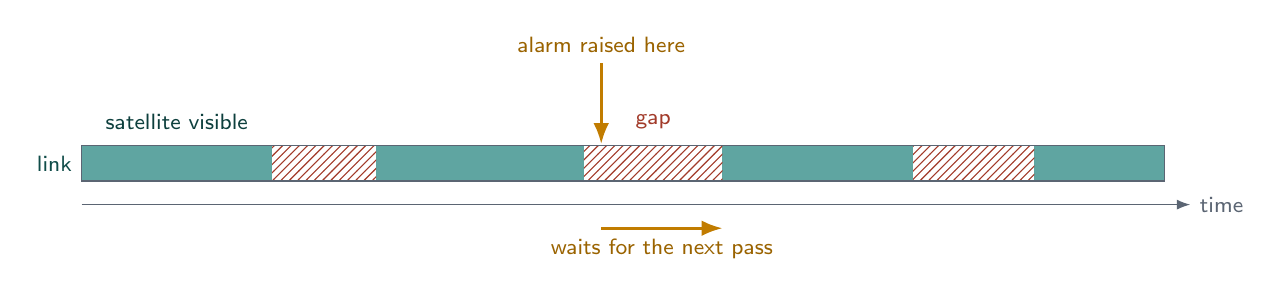
\begin{tikzpicture}[font=\sffamily\footnotesize,x=1.1cm]
\foreach \a/\b in {0/2.2, 3.4/5.8, 7.4/9.6, 11/12.5}{\fill[teal!70] (\a,0) rectangle (\b,0.45);}
\foreach \a/\b in {2.2/3.4, 5.8/7.4, 9.6/11}{\fill[pattern=north east lines,pattern color=brick] (\a,0) rectangle (\b,0.45);}
\draw[slate] (0,0) rectangle (12.5,0.45);
\node[left,teal!60!black] at (0,0.22) {link};
\draw[-{Latex},slate] (0,-0.3) -- (12.8,-0.3) node[right]{time};
\node[teal!50!black] at (1.1,0.75) {satellite visible};
\node[brick] at (6.6,0.75) {gap};
% alarm
\draw[{Latex}-,line width=1pt,amber] (6.0,0.47) -- (6.0,1.5) node[above,amber!80!black]{alarm raised here};
\draw[-{Latex},amber,line width=1pt] (6.0,-0.6) -- node[below,amber!80!black]{waits for the next pass} (7.4,-0.6);
\end{tikzpicture}
\caption{A coverage gap on a timeline. An alarm raised during a gap cannot be sent until the next satellite appears, so it misses its 100\,ms deadline by a long way.}\label{fig:gap}
\end{figure}

In the paper, the normal constellation (528 satellites) gives \emph{continuous} coverage. Thinner constellations of 240, 120 and 60 satellites create gaps: with 240 satellites, the path is covered 80\,\% of the time and gaps last 72\,s on average; with 120 satellites, only 42\,\% coverage and gaps of 336\,s.

\begin{term}{coverage}
\kt{Elevation (angle)}: how high the satellite appears above the horizon, from 0$^\circ$ (on the horizon) to 90$^\circ$ (straight overhead).\par
\kt{Elevation mask}: the minimum elevation at which a satellite is accepted (25$^\circ$ in the main runs; 15$^\circ$ and 35$^\circ$ were also tested).\par
\kt{Coverage}: the share of time that at least one usable satellite is visible.\par
\kt{Handover}: switching from one satellite to the next as they move across the sky.
\end{term}

\subsection{S2: Jamming (a physical-layer attack)}

\kt{Jamming} means deliberately transmitting radio noise on the same frequency so that the receiver cannot hear the real signal, much like someone shouting next to you while you try to listen to a friend. In the paper, a small jammer of 20\,dBm (100\,mW, similar to a Wi-Fi router) is placed 300\,m from the drone and switched on for 10 minutes.

Whether the drone can still understand the hub depends on how strong the hub's signal is compared with the noise and the jammer. This ratio is called the \kt{SINR}.

\begin{term}{radio power}
\kt{dBm}: a logarithmic unit of radio power. 0\,dBm = 1\,mW; every +10\,dB multiplies the power by 10. So 10\,dBm = 10\,mW, 20\,dBm = 100\,mW, 23\,dBm $\approx$ 200\,mW (a phone's maximum), 30\,dBm = 1\,W.\par
\kt{dB (decibel)}: the same idea for ratios. +3\,dB is roughly double, +10\,dB is ten times.\par
\kt{SINR (signal-to-interference-plus-noise ratio)}: wanted signal power divided by (unwanted interference + background noise). Higher SINR means faster, more reliable data. If it drops too low, the link fails.\par
\kt{Path loss}: how much the signal weakens as it travels. It grows with distance and frequency.\par
\kt{Antenna gain (dBi)}: how much an antenna focuses power in one direction compared with a perfect ball-shaped (isotropic) antenna.\par
\kt{EIRP}: transmit power plus antenna gain, i.e.\ the effective power sent towards the receiver. The drone's satellite terminal uses 31\,dBm + 6\,dBi = 37\,dBm EIRP.\par
\kt{Physical layer}: the lowest layer of a network, the radio waves themselves.
\end{term}

\subsection{S3: Denial-of-service flood (a network-layer attack)}

In a \kt{DoS (denial-of-service) attack}, an attacker sends a huge amount of useless traffic to block a network link. In the paper, the attacker sends 15\,Mbit/s of junk into the 10\,Mbit/s cable between the gateway and the hospital, for 10 minutes. The link can carry only 10\,Mbit/s, so packets pile up in a waiting line (a \kt{queue}) at the gateway. Jamming is also a kind of DoS, but at the radio level; the paper keeps them separate because they hit different links and need different defences.

\begin{term}{queues}
\kt{Packet}: a small chunk of data sent through a network.\par
\kt{Queue (buffer)}: a waiting line of packets in a router or device, waiting for the link to become free.\par
\kt{Drop-tail queue}: the simplest queue: when it is full, newly arriving packets are thrown away.\par
\kt{Queuing delay}: the time a packet spends waiting in the queue.\par
\kt{UDP}: a simple internet protocol that sends packets without checking that they arrived; often used for floods.
\end{term}

% ================================================================== 5
\section{Four Ways the Hub Can Behave (Policies)}

A \kt{policy} is a fixed rule for how the hub uses its radio. The paper compares four:

\begin{center}
\small
\begin{tabularx}{0.96\linewidth}{@{}>{\bfseries}p{2.9cm} p{1.2cm} X X@{}}
\toprule
Policy & Power & Order of sending & During a coverage gap \\
\midrule
P1 Max power & 23\,dBm & First come, first served & Radio stays awake \\
P2 Low power & 0\,dBm & First come, first served & Radio stays awake \\
P3 Priority & 10\,dBm & Alarms first, then ECG, then records, at the hub \emph{and} at the drone & Radio stays awake \\
P4 Store-and-forward & 10\,dBm & First come, first served & Store data and \textbf{sleep} the radio until the next satellite \\
\bottomrule
\end{tabularx}
\end{center}

\begin{figure}[h]
\centering
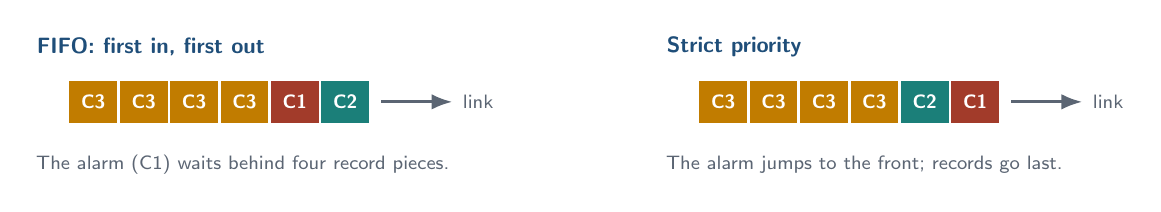
\begin{tikzpicture}[font=\sffamily\scriptsize,
  pk/.style={draw=white,minimum width=0.62cm,minimum height=0.55cm,inner sep=0,text=white,font=\sffamily\scriptsize\bfseries}]
\node[font=\sffamily\footnotesize\bfseries,navy,anchor=west] at (-0.2,1.1) {FIFO: first in, first out};
\foreach \c/\t [count=\i] in {amber/C3,amber/C3,amber/C3,amber/C3,brick/C1,teal/C2}{\node[pk,fill=\c] at (\i*0.64,0.4) {\t};}
\draw[-{Latex},line width=1pt,slate] (4.3,0.4) -- (5.2,0.4) node[right,slate]{link};
\node[anchor=west,text width=5.7cm,slate] at (-0.2,-0.4) {The alarm (C1) waits behind four record pieces.};
\begin{scope}[xshift=8.0cm]
\node[font=\sffamily\footnotesize\bfseries,navy,anchor=west] at (-0.2,1.1) {Strict priority};
\foreach \c/\t [count=\i] in {amber/C3,amber/C3,amber/C3,amber/C3,teal/C2,brick/C1}{\node[pk,fill=\c] at (\i*0.64,0.4) {\t};}
\draw[-{Latex},line width=1pt,slate] (4.3,0.4) -- (5.2,0.4) node[right,slate]{link};
\node[anchor=west,text width=5.7cm,slate] at (-0.2,-0.4) {The alarm jumps to the front; records go last.};
\end{scope}
\end{tikzpicture}
\caption{FIFO versus priority scheduling. With P3, a full drone buffer also throws out a record piece (it is re-sent later) instead of an alarm or ECG message; this is called \emph{push-out}.}\label{fig:prio}
\end{figure}

\begin{term}{policies}
\kt{Transmit power}: how strongly the hub's radio transmits. More power gives a stronger signal but uses more battery.\par
\kt{FIFO (first in, first out)}: packets are sent in the order they arrived, like a normal queue at a bank.\par
\kt{Strict priority}: urgent packets always go first, like an ambulance lane.\par
\kt{End-to-end}: applied on every hop of the path, not only at the start.\par
\kt{Store-and-forward}: keep data safely stored while no link exists, and send it when a link returns. The idea comes from \kt{delay-tolerant networking (DTN)}, used for example in deep-space communication.\par
\kt{Sleep mode}: switching the radio almost completely off to save battery.
\end{term}

% ================================================================== 6
\section{Measuring Energy}

The hub is often battery or solar powered, so its radio energy matters. A radio can be in one of three states, each drawing a different power (values from 3GPP TR~45.820, a standard model for low-power IoT radios):

\begin{center}
\small
\begin{tabular}{@{}lll@{}}
\toprule
State & Power drawn & Meaning \\
\midrule
Transmitting at 23\,dBm & 545\,mW & sending data \\
Awake and listening & 90\,mW & waiting for permission (``uplink grants'') to send \\
Deep sleep & 0.015\,mW & almost off \\
\bottomrule
\end{tabular}
\end{center}

The energy of a run is simply the power of each state multiplied by the time spent in it, summed up: $E = \sum (\text{power} \times \text{time})$, measured in \kt{joules (J)}.

\begin{example}
Over a 2-hour window (7200\,s), a hub that stays awake the whole time but transmits for only a minute or two in total spends roughly $0.09\,\text{W} \times 7200\,\text{s} \approx 650$\,J just listening. The transmissions add comparatively little. That is why P1, P2 and P3 all use 648--685\,J, almost the same, even though their transmit powers differ by a factor of 200.
\end{example}

\begin{term}{energy}
\kt{Uplink grant}: a short message in which the base station (here, the drone) tells the device ``you may transmit now, in this time slot''. A connected device must keep listening for these.\par
\kt{Joule (J)}: the unit of energy; 1\,J = 1\,W for 1\,s.\par
\kt{Idle power}: the power drawn while awake but not transmitting. Because it is uncertain for real devices, the paper also repeats the analysis with 3, 20 and 90\,mW.\par
\kt{Relative power units (TR 38.840)}: the 5G standard's power model gives values relative to deep sleep (sleep = 1, listening = 100, transmitting = 250--700) rather than in watts.
\end{term}

% ================================================================== 7
\section{A Simple Formula for Missed Alarms}\label{sec:model}

One of the paper's contributions is a short formula that predicts how many alarms will be late, \emph{without} running a simulation. The reasoning is surprisingly simple.

\textbf{Step 1.} Suppose a gap lasts $G$ seconds. An alarm that arrives $u$ seconds after the gap began must wait $G-u$ seconds for the next satellite.

\textbf{Step 2.} It misses its deadline $\tau$ (100\,ms) if this wait plus the normal delay $\delta$ is larger than $\tau$. Nearly every alarm raised during a gap therefore misses, except those raised in the last $(\tau-\delta)$ seconds before the satellite appears.

\textbf{Step 3.} Alarms occur at random times that have nothing to do with where the satellites are. So the \emph{share of alarms} that fall into gaps equals the \emph{share of time} taken up by gaps. (This is a well-known property of random arrivals.)

Putting the steps together, with $G_i$ the length of gap $i$ and $T$ the total observation time:

\begin{tcolorbox}[colback=white,colframe=navy,arc=2pt,boxrule=0.8pt]
\begin{align*}
P_\text{miss}(\tau) &\approx \frac{1}{T}\sum_i \bigl(G_i-(\tau-\delta)\bigr)^{+}
&&\text{(share of alarms that miss the deadline)}\\[4pt]
\mathbb{E}[W] &= \frac{1}{2T}\sum_i G_i^{2}
&&\text{(average extra waiting time)}
\end{align*}
\end{tcolorbox}

The symbol $(x)^+$ means ``$x$ if positive, otherwise 0'', and $\mathbb{E}[W]$ is the expected (average) waiting time.

\begin{example}
Take a 2-hour window ($T = 7200$\,s) with five gaps of $G = 300$\,s each, a deadline $\tau = 0.1$\,s and normal delay $\delta = 0.01$\,s.
\[
P_\text{miss} \approx \frac{5\times(300-0.09)}{7200} \approx 0.208 = 20.8\,\%,\qquad
\mathbb{E}[W] = \frac{5\times300^2}{2\times7200} \approx 31\,\text{s}.
\]
About one alarm in five is late, which is almost exactly the 1\,500\,s of gaps divided by 7\,200\,s. Notice that the transmit power appears nowhere in the formula.
\end{example}

Two lessons follow directly from the formula. First, for a deadline of 0.1\,s and gaps of minutes, the miss rate is simply the \emph{fraction of time without coverage}; no amount of transmit power can fix it. Second, the waiting time grows with the \emph{square} of the gap length, so a few long gaps are much worse than many short ones.

The paper tested the formula against 40 simulation runs: the prediction was off by only 1.8 percentage points on average (correlation 0.997), and it kept working when the elevation mask was changed between 15$^\circ$ and 35$^\circ$.

\begin{term}{statistics and modelling}
\kt{Closed-form model}: a formula you can evaluate directly, as opposed to a simulation.\par
\kt{Mean absolute error (MAE)}: the average size of the difference between prediction and simulation.\par
\kt{Correlation}: a number from $-1$ to $+1$ telling how closely two quantities move together; 0.997 means almost perfectly.\par
\kt{Percentage point (pp)}: the difference between two percentages, e.g.\ from 20\,\% to 22\,\% is 2 percentage points.\par
\kt{Assumption}: a condition under which the model is valid. Here: alarms are independent of the gaps, delay during coverage is small, the load is light, and gaps come only from satellite geometry.
\end{term}

% ================================================================== 8
\section{How the Experiments Were Done}

Building a real drone-satellite-hospital system with attackers would be expensive and unsafe, so the paper uses \kt{simulation}: a computer program that imitates every device and every packet.

\begin{itemize}
\item \textbf{Simulator.} \kt{ns-3}, a free and widely used network simulator in research. Two versions of the scenario were built:
  \begin{itemize}
  \item a \kt{system-level} version, in which the hub-drone radio is described by a simplified formula (signal strength $\rightarrow$ data rate); fast, good for many runs;
  \item a \kt{full 5G NR} version using \kt{5G-LENA}, an add-on that simulates the real 5G protocol: scheduling, retransmissions and automatic speed adjustment. It is slower but more realistic.
  \end{itemize}
\item \textbf{Satellites.} Real orbital motion; every second the program checks which satellites are above the mask for both the drone and the gateway, and picks the highest one.
\item \textbf{Standards.} The radio models, power values and targets all come from 3GPP documents. As a check, the satellite link calculation reproduced the published 3GPP TR~38.821 values within 0.04\,dB.
\item \textbf{Repetitions.} Each case was run 10 times with different random \kt{seeds} (5 for the extra sensitivity runs), and results are reported as an average with a \kt{95\,\% confidence interval}.
\end{itemize}

\begin{term}{simulation}
\kt{Abstraction}: a simplified model that keeps the important behaviour but leaves out details.\par
\kt{Shannon rate}: the theoretical maximum data rate for a given SINR and bandwidth; the system-level model uses a slightly reduced (``attenuated'') version of it.\par
\kt{Link budget}: an accounting of all gains and losses on a radio link, used to check that the signal arrives strong enough.\par
\kt{Bandwidth}: the width of the radio channel (e.g., 1\,MHz or 10\,MHz). More bandwidth carries more data.\par
\kt{Retransmission (HARQ)}: automatically resending a packet that arrived damaged.\par
\kt{Random seed}: the starting number of the simulator's random generator. Different seeds give different but equally valid ``worlds'' (different satellite positions, fading, alarm times).\par
\kt{Confidence interval (95\,\%)}: a range around the average that likely contains the true value; a narrow range means the result is reliable.\par
\kt{Reproducible}: anyone can repeat the experiment and get the same numbers. All code and data are public (see Further Reading).
\end{term}

% ================================================================== 9
\section{What the Paper Found: Six Lessons}

\subsection{Lesson 1: The satellites, not the hub, decide whether alarms are on time}

\begin{figure}[h]
\centering
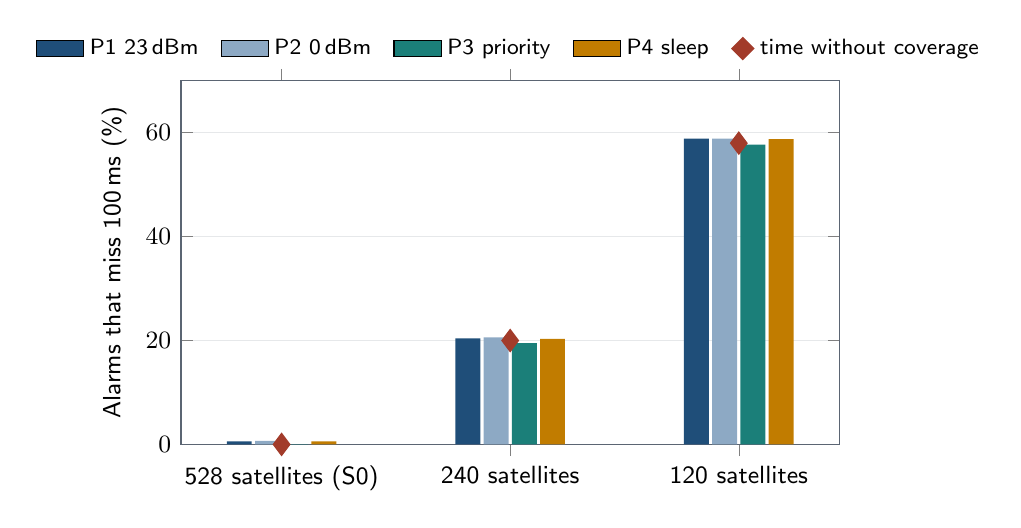
\begin{tikzpicture}
\begin{axis}[
  width=0.82\linewidth,height=6.2cm,
  ybar=1.2pt,bar width=9pt,area legend,
  ymin=0,ymax=70,
  symbolic x coords={528 satellites (S0),240 satellites,120 satellites},
  xtick=data,
  enlarge x limits=0.22,
  ylabel={Alarms that miss 100\,ms (\%)},
  ylabel style={font=\sffamily\small},
  tick label style={font=\sffamily\small},
  legend style={font=\sffamily\footnotesize,draw=none,fill=none,legend columns=5,at={(0.5,1.03)},anchor=south,/tikz/every even column/.append style={column sep=6pt}},
  axis line style={slate},
  ymajorgrids,grid style={slate!15},
  nodes near coords style={font=\sffamily\tiny},
]
\addplot[fill=cP1,draw=none] coordinates {(528 satellites (S0),0.60) (240 satellites,20.40) (120 satellites,58.85)};
\addplot[fill=cP2,draw=none] coordinates {(528 satellites (S0),0.69) (240 satellites,20.62) (120 satellites,58.89)};
\addplot[fill=cP3,draw=none] coordinates {(528 satellites (S0),0.04) (240 satellites,19.49) (120 satellites,57.70)};
\addplot[fill=cP4,draw=none] coordinates {(528 satellites (S0),0.60) (240 satellites,20.32) (120 satellites,58.76)};
\addplot[only marks,mark=diamond*,mark size=4pt,brick,legend image code/.code={\node[diamond,fill=brick,inner sep=1.8pt] at (0.15cm,0) {};}] coordinates {(528 satellites (S0),0) (240 satellites,20) (120 satellites,58)};
\legend{P1 23\,dBm,P2 0\,dBm,P3 priority,P4 sleep,time without coverage}
\end{axis}
\end{tikzpicture}
\caption{Alarm deadline misses (mean of 10 seeds) for each policy and constellation size. All four policies miss almost exactly the share of time without coverage (red diamonds), whatever their transmit power.}\label{fig:lesson1}
\end{figure}

With continuous coverage, the best policy (P3) missed only 0.04\,\% of alarms and 0.07\,\% of ECG messages. With 240 satellites, every policy missed about 20\,\% of alarms, and with 120 satellites about 58\,\%. Alarms raised during a gap had to wait for the next pass: the slowest 5\,\% of alarms waited about a minute with 240 satellites and about five and a half minutes with 120 satellites.

\insight{If the constellation leaves gaps, no hub setting can save the alarms. Either the constellation must be dense enough (or the mask low enough), or alarms need a second path, such as a terrestrial or messaging fallback.}

A note on honesty with statistics: with continuous coverage, P3 had \emph{zero} failures in about 1.44 million ECG messages. That sounds perfect, but the \kt{rule of three} says that zero failures in $n$ trials only shows, with 95\,\% confidence, that the failure rate is below $3/n \approx 2.1\times10^{-6}$. That is consistent with the ``six nines'' target but does not prove it; proving it would need roughly three times as many failure-free messages. Good research states such limits openly.

\subsection{Lesson 2: Sleeping saves energy; lowering power hardly does}

\begin{figure}[h]
\centering
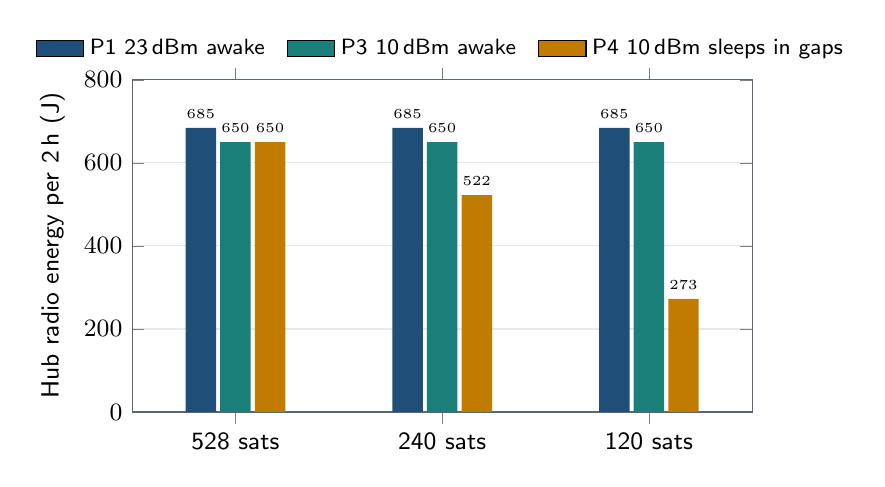
\begin{tikzpicture}
\begin{axis}[
  width=0.78\linewidth,height=5.8cm,
  ybar=1.5pt,bar width=11pt,area legend,
  ymin=0,ymax=800,
  symbolic x coords={528 sats,240 sats,120 sats},
  xtick=data,enlarge x limits=0.25,
  ylabel={Hub radio energy per 2\,h (J)},
  ylabel style={font=\sffamily\small},
  tick label style={font=\sffamily\small},
  legend style={font=\sffamily\footnotesize,draw=none,fill=none,legend columns=3,at={(0.5,1.03)},anchor=south,/tikz/every even column/.append style={column sep=6pt}},
  axis line style={slate},ymajorgrids,grid style={slate!15},
  nodes near coords,nodes near coords style={font=\sffamily\tiny,/pgf/number format/fixed,/pgf/number format/precision=0},
]
\addplot[fill=cP1,draw=none] coordinates {(528 sats,684.5) (240 sats,684.5) (120 sats,684.5)};
\addplot[fill=cP3,draw=none] coordinates {(528 sats,649.8) (240 sats,649.8) (120 sats,649.8)};
\addplot[fill=cP4,draw=none] coordinates {(528 sats,649.8) (240 sats,522.1) (120 sats,272.5)};
\legend{P1 23\,dBm awake,P3 10\,dBm awake,P4 10\,dBm sleeps in gaps}
\end{axis}
\end{tikzpicture}
\caption{Hub radio energy. Going from 23\,dBm to 10\,dBm saves only 5\,\%, but sleeping during gaps (P4) saves 20\,\% at 240 satellites and 58\,\% at 120 satellites, without missing more alarms.}\label{fig:energy}
\end{figure}

Because a connected radio spends most of its time listening (Section~6), lowering the transmit power changes little. P4, which simply switches the radio off when no satellite is visible, used 20\,\%, 58\,\% and 85\,\% less energy than P3 at 240, 120 and 60 satellites, and it missed the same alarms as the always-awake policies: a free saving. This held for any idle power between 3 and 90\,mW.

\insight{On a link with gaps, the most effective way to save battery is to sleep through the gaps, not to whisper.}

\subsection{Lesson 3: Under jamming, only maximum power survives (for a while)}

\begin{figure}[h]
\centering
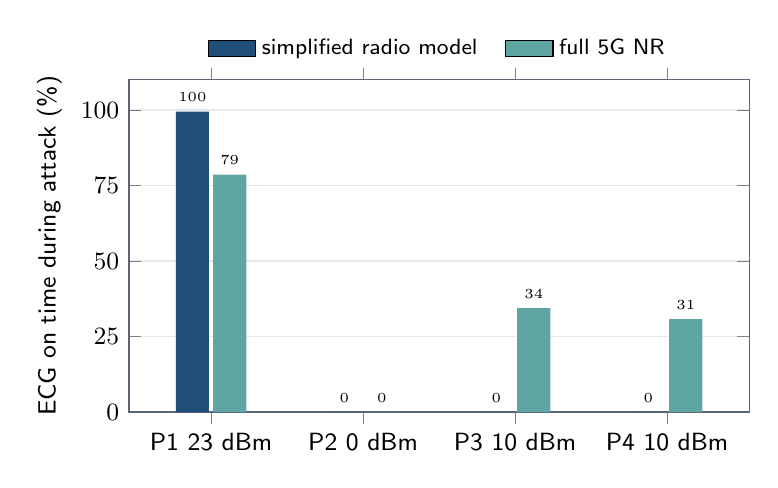
\begin{tikzpicture}
\begin{axis}[
  width=0.78\linewidth,height=5.8cm,
  ybar=1.5pt,bar width=12pt,area legend,
  ymin=0,ymax=110,ytick={0,25,50,75,100},
  symbolic x coords={P1 23 dBm,P2 0 dBm,P3 10 dBm,P4 10 dBm},
  xtick=data,enlarge x limits=0.18,
  ylabel={ECG on time during attack (\%)},
  ylabel style={font=\sffamily\small},
  tick label style={font=\sffamily\small},
  legend style={font=\sffamily\footnotesize,draw=none,fill=none,legend columns=2,at={(0.5,1.03)},anchor=south,/tikz/every even column/.append style={column sep=8pt}},
  axis line style={slate},ymajorgrids,grid style={slate!15},
  nodes near coords,nodes near coords style={font=\sffamily\tiny,/pgf/number format/fixed,/pgf/number format/precision=0},
]
\addplot[fill=navy,draw=none] coordinates {(P1 23 dBm,99.5) (P2 0 dBm,0) (P3 10 dBm,0) (P4 10 dBm,0)};
\addplot[fill=teal!70,draw=none] coordinates {(P1 23 dBm,78.6) (P2 0 dBm,0) (P3 10 dBm,34.4) (P4 10 dBm,30.8)};
\legend{simplified radio model,full 5G NR}
\end{axis}
\end{tikzpicture}
\caption{Share of ECG messages on time while a 20\,dBm jammer is active (matched 30-min runs, mean of 10 seeds). The full 5G stack fights back with retransmissions and slower but robust coding, so its picture is less black-and-white.}\label{fig:jam}
\end{figure}

Against the reference jammer, only the 23\,dBm policy kept the ECG stream usable. The 10\,dBm and 0\,dBm hubs were drowned out. In the full 5G simulation, the result also varied strongly from seed to seed: in some ``worlds'' the hub survived and in others it was cut off completely. This is why the paper reports every seed, not just the average: an average can hide a case in which a patient is left unmonitored.

The sensitivity runs (Lesson~6) show that P1's advantage is only a \emph{power margin}: a jammer 7--10\,dB stronger than the hub silences any fixed policy.

\subsection{Lesson 4: A DoS flood mostly makes messages late, not lost}

\begin{figure}[h]
\centering
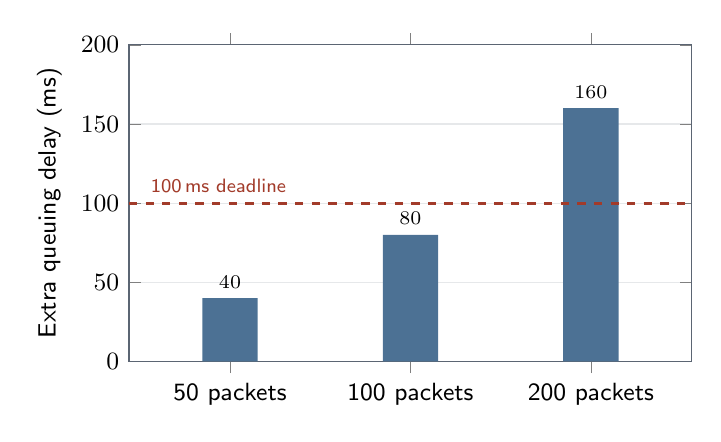
\begin{tikzpicture}
\begin{axis}[
  width=0.72\linewidth,height=5.6cm,
  ybar,bar width=20pt,
  ymin=0,ymax=200,
  symbolic x coords={50 packets,100 packets,200 packets},
  xtick=data,enlarge x limits=0.28,
  ylabel={Extra queuing delay (ms)},
  ylabel style={font=\sffamily\small},
  tick label style={font=\sffamily\small},
  axis line style={slate},ymajorgrids,grid style={slate!15},
  nodes near coords,nodes near coords style={font=\sffamily\scriptsize},
]
\addplot[fill=navy!80,draw=none] coordinates {(50 packets,40) (100 packets,80) (200 packets,160)};
\draw[brick,dashed,line width=1pt] (rel axis cs:0,0.5) -- (rel axis cs:1,0.5) node[pos=0.02,above,anchor=south west,font=\sffamily\scriptsize,brick]{100\,ms deadline};
\end{axis}
\end{tikzpicture}
\caption{Delay added by a full gateway queue of $B$ packets of 1\,kB on a 10\,Mbit/s link: $B\times L/C$. With 200 packets the queue alone exceeds the deadline.}\label{fig:dos}
\end{figure}

When the flood fills the gateway queue, every patient message has to wait behind it. The extra delay is roughly
\[
\text{delay} \approx \frac{B\times L}{C} = \frac{\text{queue length (packets)}\times\text{packet size (bits)}}{\text{link rate (bit/s)}}.
\]
\begin{example}
For the reference queue of $B = 100$ packets of $L = 1$\,kB $= 8000$\,bits on $C = 10$\,Mbit/s: delay $= 100\times8000/10^7 = 0.08$\,s $= 80$\,ms. Add the normal 10--30\,ms of path delay and the ECG messages are right at the 100\,ms limit.
\end{example}

With a 50-packet queue, 99\,\% of ECG messages stayed on time; with 200 packets, none did, yet 99.95--99.99\,\% still arrived within the 1.1\,s survival time. In other words, the flood ``eats'' the time budget but does not cut the stream.

\insight{Against a flood at the gateway, keep the queue small enough to drain within the deadline, or let patient traffic bypass the queue with priority.}

\subsection{Lesson 5: Priority only helps if every hop applies it}

\begin{figure}[h]
\centering
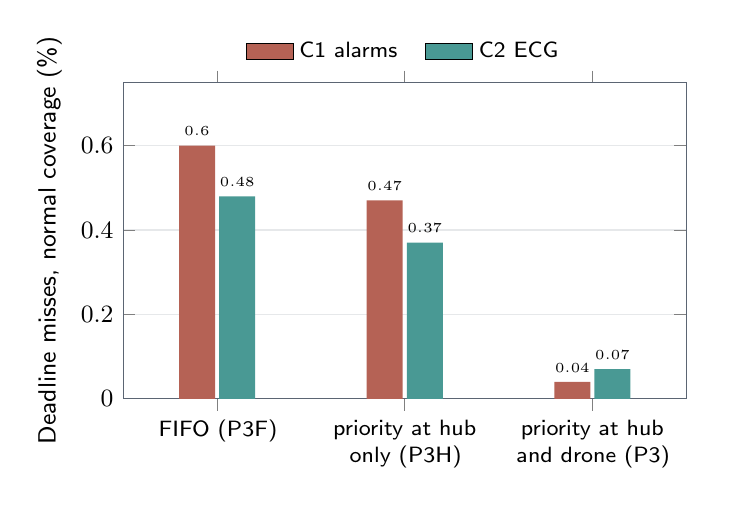
\begin{tikzpicture}
\begin{axis}[
  width=0.72\linewidth,height=5.6cm,
  ybar=1.5pt,bar width=13pt,area legend,
  ymin=0,ymax=0.75,
  symbolic x coords={FIFO (P3F),priority at hub only (P3H),priority at hub and drone (P3)},
  xtick=data,enlarge x limits=0.25,
  x tick label style={font=\sffamily\footnotesize,text width=2.6cm,align=center},
  ylabel={Deadline misses, normal coverage (\%)},
  ylabel style={font=\sffamily\small},
  y tick label style={font=\sffamily\small},
  legend style={font=\sffamily\footnotesize,draw=none,fill=none,legend columns=2,at={(0.5,1.03)},anchor=south,/tikz/every even column/.append style={column sep=8pt}},
  axis line style={slate},ymajorgrids,grid style={slate!15},
  nodes near coords,nodes near coords style={font=\sffamily\tiny,/pgf/number format/fixed,/pgf/number format/precision=2},
]
\addplot[fill=brick!80,draw=none] coordinates {(FIFO (P3F),0.60) (priority at hub only (P3H),0.47) (priority at hub and drone (P3),0.04)};
\addplot[fill=teal!80,draw=none] coordinates {(FIFO (P3F),0.48) (priority at hub only (P3H),0.37) (priority at hub and drone (P3),0.07)};
\legend{C1 alarms,C2 ECG}
\end{axis}
\end{tikzpicture}
\caption{The priority ablation: all three variants use 10\,dBm and stay awake, so only the scheduling differs. Most of the gain comes from applying priority at the drone, where alarms otherwise queue behind record pieces.}\label{fig:abl}
\end{figure}

To be sure that it really is the \emph{priority} that helps (and not the power or the sleep), the paper ran an \kt{ablation}: it switched features on and off one at a time, keeping everything else equal. Priority at the hub alone helped a little; priority at the drone as well cut ECG misses from 0.48\,\% to 0.07\,\%. During gaps or jamming, however, priority changed the miss rate by at most about one percentage point, because no ordering can deliver data over a link that does not exist.

\begin{term}{evaluation methods}
\kt{Ablation study}: removing or changing one component at a time to measure its individual effect.\par
\kt{Sensitivity analysis}: repeating the experiment with different settings (e.g., jammer power) to see whether the conclusions still hold.\par
\kt{Baseline}: a simple reference method that a new method is compared against. The four fixed policies are baselines for a future smart controller.
\end{term}

\subsection{Lesson 6: The ranking is stable, but survival depends on attack strength}

\begin{figure}[h]
\centering
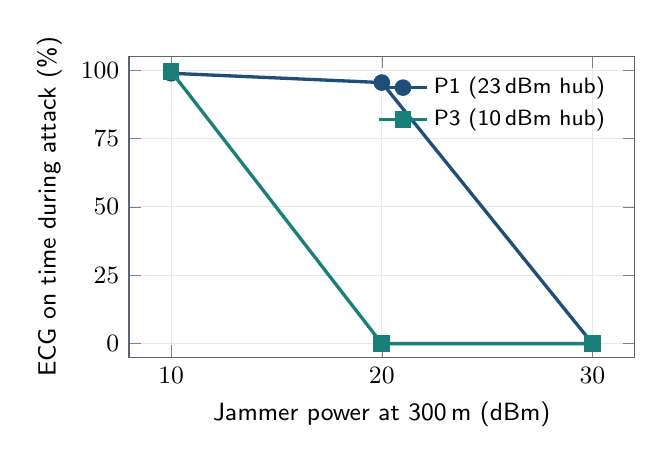
\begin{tikzpicture}
\begin{axis}[
  width=0.66\linewidth,height=5.4cm,
  xmin=8,xmax=32,xtick={10,20,30},
  ymin=-5,ymax=105,ytick={0,25,50,75,100},
  xlabel={Jammer power at 300\,m (dBm)},
  ylabel={ECG on time during attack (\%)},
  label style={font=\sffamily\small},tick label style={font=\sffamily\small},
  legend style={font=\sffamily\footnotesize,draw=none,fill=none,at={(0.97,0.97)},anchor=north east},
  axis line style={slate},grid=major,grid style={slate!15},
]
\addplot[cP1,line width=1.2pt,mark=*,mark size=2.4pt] coordinates {(10,98.9) (20,95.5) (30,0)};
\addplot[cP3,line width=1.2pt,mark=square*,mark size=2.4pt] coordinates {(10,99.6) (20,0) (30,0)};
\legend{P1 (23\,dBm hub),P3 (10\,dBm hub)}
\end{axis}
\end{tikzpicture}
\caption{Sensitivity to jammer power (simplified model, mean of 5 seeds). Each hub survives a jammer of roughly its own power and fails once the jammer is clearly stronger.}\label{fig:sens}
\end{figure}

The extra runs changed one assumption at a time: jammer power (10/20/30\,dBm) and distance (150/300/600\,m), flood rate (11/15/20\,Mbit/s), gateway queue size (50/100/200 packets) and elevation mask (15/25/35$^\circ$). The order of the policies never changed, but whether \emph{any} fixed policy survived depended on how strong the attack was. Lowering the mask to 15$^\circ$ closed every gap of the 240-satellite constellation, while raising it to 35$^\circ$ halved the coverage, and the formula of Section~\ref{sec:model} still matched the simulation (correlation 0.995).

% ================================================================== 10
\section{So, Is It Feasible?}

\begin{center}
\small
\begin{tabularx}{0.96\linewidth}{@{}>{\bfseries}l >{\centering\arraybackslash}p{1.4cm} X@{}}
\toprule
Situation & Feasible? & Condition \\
\midrule
Routine monitoring, dense constellation & \textcolor{teal}{\textbf{Yes}} & Continuous coverage, priority on every hop, protected gateway. \\
Records over a sparse constellation & \textcolor{teal}{\textbf{Yes}} & Store and forward works down to 120 satellites; at 60 satellites only half the records complete. \\
Emergency alarms over a sparse constellation & \textcolor{brick}{\textbf{No}} & Misses equal the time without coverage; a second path is needed. \\
Strong or nearby jammer & \textcolor{brick}{\textbf{No}} & Needs power headroom, frequency hopping or jamming detection with fallback. \\
DoS flood at the gateway & \textcolor{amber}{\textbf{Partly}} & Messages arrive late, not lost; fix with priority queuing or a smaller queue. \\
\bottomrule
\end{tabularx}
\end{center}

The overall message is that \emph{every fixed policy fails somewhere}: P1 survives jamming but wastes energy, P4 saves energy but has no defence against attacks, and P3 protects alarms only while the link survives. This motivates the next step of the research: an \kt{adaptive controller}, possibly based on machine learning, that watches satellite visibility, link quality and queues, and changes power, priority and sleep on the fly.

% ================================================================== 11
\section{Limitations: What the Paper Does Not Claim}

Stating limitations is a sign of good science, not of weakness. The paper is careful to say that:
\begin{itemize}
\item all results come from simulation, with one drone and one constellation shell;
\item ``clinical resilience'' is meant in a \emph{communication} sense: meeting targets that 3GPP derived from clinical needs. Whether that is enough for safe patient care must be checked with clinicians;
\item the attacks are one type of jammer and one type of queue, tested over the ranges listed above;
\item handover signalling and the satellite-to-gateway link are simplified, and the energy covers only the hub's radio, not the sensors, drone or satellite.
\end{itemize}

% ================================================================== 12
\section{Glossary}\label{sec:glossary}

\begin{multicols}{2}\small
\begin{description}[font=\sffamily\bfseries\color{navy},leftmargin=0pt,itemsep=0.15em]
\item[3GPP] Body that writes mobile-network standards; its reports are TRs, its specifications TSs.
\item[5G NR] The radio technology of 5G (``New Radio'').
\item[5G-LENA] Add-on to ns-3 that simulates the full 5G NR protocol.
\item[Ablation] Changing one component at a time to measure its effect.
\item[Availability] Share of time the service works; ``six nines'' = 99.9999\,\%.
\item[Backhaul] Long-distance link from a local network to the core or hospital.
\item[Bandwidth] Width of a radio channel (Hz); more bandwidth, more data.
\item[Bent pipe] Satellite that only amplifies and forwards the signal.
\item[Confidence interval] Range around a mean that likely contains the true value.
\item[Constellation (shell)] Group of satellites at one altitude covering the Earth.
\item[Coverage gap] Period with no usable satellite in view.
\item[dB, dBm] Logarithmic units for ratios and for power relative to 1\,mW.
\item[Deadline miss] A message that arrives later than its deadline.
\item[DoS] Denial-of-service attack: flooding a link to block real traffic.
\item[Drop-tail queue] Queue that discards new packets when full.
\item[ECG] Electrical signal of the heart.
\item[EIRP] Transmit power plus antenna gain.
\item[Elevation, mask] Angle of a satellite above the horizon; minimum accepted angle.
\item[FIFO] First in, first out scheduling.
\item[Gateway (ground)] Satellite dish that receives data back from space.
\item[Handover] Switching from one satellite (or cell) to the next.
\item[Hub] Clinic box collecting all sensor data.
\item[IoMT] Internet of Medical Things.
\item[Jamming] Transmitting noise to block a radio link.
\item[Latency] Time from sending to arrival.
\item[LEO] Low Earth orbit (a few hundred km).
\item[Link budget] Accounting of gains and losses on a radio link.
\item[ns-3] Open-source network simulator.
\item[Packet] Small chunk of data sent over a network.
\item[Path loss] Weakening of a signal with distance.
\item[Percentage point] Difference between two percentages.
\item[Poisson process] Model of random, independent events.
\item[Policy] Fixed rule for how the hub uses its radio.
\item[Priority (strict)] Urgent packets always sent first.
\item[Queue] Waiting line of packets.
\item[Rule of three] Zero failures in $n$ trials $\Rightarrow$ failure rate below $3/n$ (95\,\%).
\item[SAGIN] Space-air-ground integrated network.
\item[Seed] Starting number for the simulator's randomness.
\item[Sensitivity analysis] Repeating experiments with changed settings.
\item[SINR] Signal-to-interference-plus-noise ratio.
\item[Store-and-forward] Keep data while no link exists, send when it returns.
\item[Survival time] How long an application tolerates a missing message.
\item[UAV] Unmanned aerial vehicle (drone).
\item[Uplink grant] Base-station permission for a device to transmit.
\item[Walker-delta] Standard evenly spaced satellite constellation design.
\end{description}
\end{multicols}

% ================================================================== 13
\section{Check Your Understanding}\label{sec:quiz}

\begin{enumerate}[label=\textbf{Q\arabic*.}]
\item Why does increasing the hub's transmit power not reduce alarm misses when the constellation has 120 satellites?
\item A constellation has gaps that cover 30\,\% of the time. Roughly what share of alarms will miss a 100\,ms deadline?
\item Which is worse for the average waiting time: ten gaps of 60\,s or one gap of 600\,s? Use $\mathbb{E}[W]=\sum G_i^2/(2T)$.
\item Convert 20\,dBm and 30\,dBm to milliwatts.
\item A gateway queue holds 150 packets of 1\,kB on a 10\,Mbit/s link. What extra delay does a full queue add? Is the 100\,ms deadline still achievable?
\item Why did P4 save energy at 240 satellites but not at 528 satellites?
\item Why does the paper report the result of every seed under jamming, and not only the average?
\item What is the difference between an ablation study and a sensitivity analysis?
\end{enumerate}

\textsf{\textbf{Answers.}}\small
\textbf{Q1:} During a gap there is no satellite at all, so there is nothing to transmit to; power cannot create a link.
\textbf{Q2:} About 30\,\%, the share of time without coverage.
\textbf{Q3:} Both total 600\,s of gaps, but $\sum G_i^2$ is $10\times3600 = 36\,000$ against $360\,000$: the single long gap gives ten times the average wait.
\textbf{Q4:} 100\,mW and 1000\,mW (1\,W).
\textbf{Q5:} $150\times8000/10^7 = 0.12$\,s = 120\,ms, already above the deadline before any other delay.
\textbf{Q6:} With 528 satellites there are no gaps, so P4 never gets a chance to sleep.
\textbf{Q7:} The outcome is all-or-nothing per seed; an average of, say, 50\,\% could hide a case where a patient receives no monitoring at all.
\textbf{Q8:} An ablation switches \emph{components of the method} on and off; a sensitivity analysis changes \emph{conditions or assumptions} (attack strength, queue size, mask) to test whether conclusions still hold.
\normalsize

% ================================================================== 14
\section{Further Reading}

\begin{itemize}
\item The paper itself: SUNRISE 2026, Springer CCIS (in press). Code and data:\\ \url{https://github.com/MIYM5/sagin-iomt-resilience}.
\item M.\,I.\ Younas, M.\,J.\ Iqbal, A.\ Aziz and A.\,H.\ Sodhro, ``Toward QoS Monitoring in IoT Edge Devices Driven Healthcare: A Systematic Literature Review,'' \emph{Sensors}, vol.~23, no.~21, 8885, 2023: why healthcare QoS should be judged against clinical targets.
\item M.\,I.\,Y.\ Mughal, A.\,H.\ Sodhro and M.\ Johnsson, ``A Systematic Review of Experimentally Validated Authentication Schemes for 5G/6G Smart Healthcare Edge Devices,'' SUNRISE 2025, Springer CCIS, vol.~2867, pp.~34--50, 2026: the security side of the same healthcare edge devices.
\item 3GPP TR~22.826, ``Study on communication services for critical medical applications'': the source of the 100\,ms and 1\,s targets.
\item The ns-3 tutorial (\texttt{nsnam.org}) and the 5G-LENA documentation, for students who want to run the simulations themselves.
\end{itemize}

\end{document}
